The system can be configured using the GUI. Available configuration settings is checkpoint circles, door mask area, exclusion mask and grayscale height threshold settings. 

The circles should be placed so persons walking into the room inevitable will pass all three lines. They should also be more inside the room compared to the door mask area. A good placement is illustrated in figure \ref{fig:circlePlacement}. Note that the red, most inner circle, includes the upper corners of the door frame. A too small inner circle will cause people to miss it and will therefore not be detected. 

\begin{figure}[H]
	\centering
	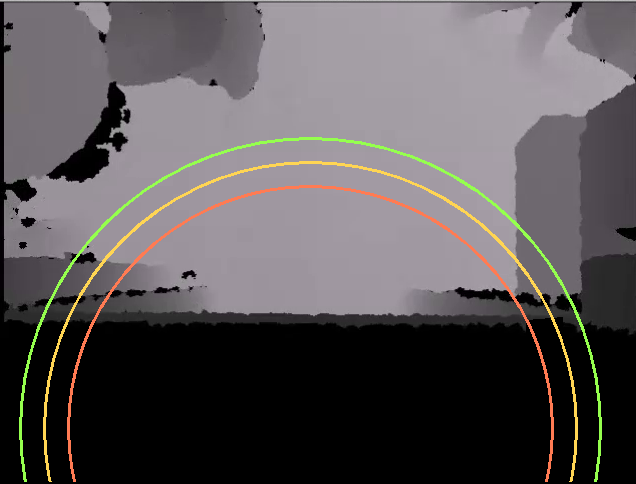
\includegraphics[width=\linewidth]{images/Manual2.png}
	\caption[Circle placment]{\textit{A prefered placement of the circles. }}
	\label{fig:circlePlacement}  %Skapar referens till figuren
\end{figure}

\newpage
The door mask should cover the area close to the door where people appear. It is important to make this area big enough, rather too big than too small. It can, but should not cover the upper, most distant, part of the red circle, figure \ref{fig:doorMask} illustrates this.

\begin{figure}[H]
	\centering
	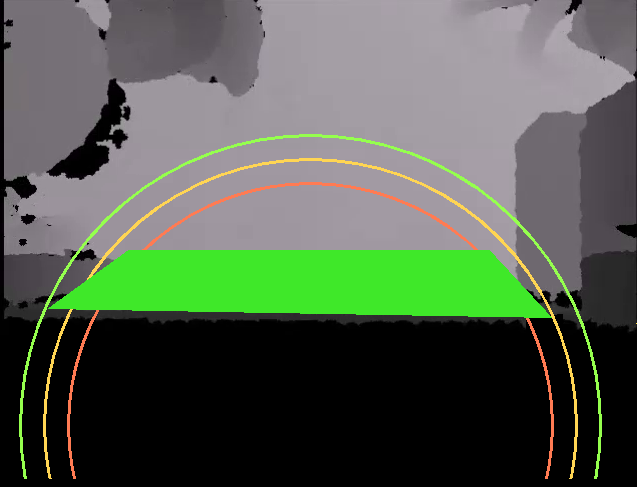
\includegraphics[width=\linewidth]{images/Manual3.png}
	\caption[Exclusion mask]{\textit{The prefered placement of the door mask, the door mask is the green area.}}
	\label{fig:doorMask}  %Skapar referens till figuren
\end{figure}

\newpage
Exclusion masks should cover areas where people can not walk or appear. This could be areas like tables or areas behind the door (walls in this case), figure \ref{fig:exMask} illustrates this. Note that for long usage of the system, movable furniture should not be excluded.

\begin{figure}[H]
	\centering
	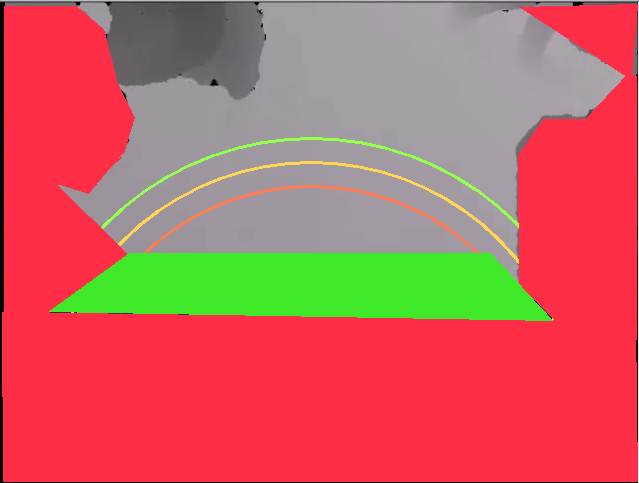
\includegraphics[width=\linewidth]{images/Manual1.png}
	\caption[Exclusion mask]{\textit{Exclusion mask is marked as red. It covers areas where people can not walk or appear.}}
	\label{fig:exMask}  %Skapar referens till figuren
\end{figure}